	\chapter{Association schemes}\label{association}
	Association schemes arise in group theory, graph theory, design theory, coding theory and more. For example, let $X$ be a finite group with conjugacy classes $\cC[g] = \{hgh^{-1}:h\in X\}$ ($g\in X$). We may form relations on the pairs of group elements via $R_g = \left\{ (a,b) \mid ab^{-1} \in \cC[g]  \right\}$; in this way, each conjugacy class results in a single relation independent of the representative group element chosen. We may then merge the relations $R_g\cup R_{g^{-1}}$ to arrive at symmetric relations. The group, along with the relations, then form a $d$-class association scheme where $d$ is the number of non-trivial relations formed (relations other than $R_e$ for identity element $e$). While we may easily construct such an association scheme from a group, we find that there are many more association schemes which do not require the group structure on the point set. In fact, for any finite set $X$, the orbits on $X\times X$ of any 
	permutation group $\mathcal{G}$ acting generously transitively (for any two points in $X$, there exists a group element swapping these elements) also gives an association scheme.
	Some of the most well-studied association schemes are distance-regular graphs, including Moore graphs, distance-transitive graphs, strongly regular graphs, generalized polygons, etc.  For an introduction to the 
	extensive literature on the subject, the reader may consult \cite{Delsarte1973,Bannai1984,Brouwer1989,Godsil1993}, 
	the survey \cite{Martin2009}, or the more recent book of  Bailey \cite{Bailey2004} which focuses on 
	connections to the statistical design of experiments.
	\begin{definition}
	Let $X$ be a finite set of vertices. A \textit{symmetric d-class association scheme}\index{association scheme!symmetric} (see \cite{Brouwer1989}) on $X$ is a pair $(X,\mathcal{R})$ where $\mathcal{R} =\left\{R_0,R_1,\dots,R_d\right\}$ is a set of $d+1$ relations on $X$ satisfying the following properties:
	\begin{enumerate}[label=$(\roman*)$]
		\item $R_0$ is the identity relation;
		\item $\left\{R_0,R_1,\dots, R_d\right\}$ forms a partition of $X\times X$;
		\item $(x,y)\in R_i$ implies $(y,x)\in R_i$;
		\item for $0\leq i,j,k\leq d$ there exist constants $p_{i,j}^k$ such that for any vertices $x,y\in X$ with $(x,y)\in R_k$, the number of vertices $z$ for which $(x,z)\in R_i$ and $(z,y)\in R_j$ is $p_{i,j}^k$, depending only on $i$, $j$, and $k$.
	\end{enumerate}
	\end{definition}
	The constants $p_{i,j}^k$ are known as the \emph{intersection numbers}\index{parameters!intersection numbers} of our association scheme and we allow ourselves to suppress the comma whenever $i$ and $j$ are given by single digits, thus $p_{5,2}^7$ and $p_{52}^7$ are synonymous throughout this thesis. Properties \emph{(iii)} and \emph{(iv)} together imply that $p_{ij}^k = p_{ji}^k$ for all $i,j,k$; we call such an association scheme \textit{commutative}. There is a broader definition for a \emph{commutative association scheme}\index{association scheme!commutative} where we replace \emph{(iii)} with the condition that for every $i$, there exists some $i'$ such that $R_{i'} = R_i^T$; that is $(x,y)\in R_i$ if and only if $(y,x)\in R_{i'}$. In this case however, we add the property $p_{ij}^k = p_{ji}^k$. Throughout this thesis, all association schemes will be symmetric, though we will add remarks at times when the theorems apply directly to the non-symmetric case as well.
	
	For each $0\leq i\leq d$ we define the (undirected) graph $\Gamma_i = \Gamma(X,R_i)$ on $X$ with $\Gamma_1,\dots,\Gamma_d$ all simple. Note, throughout this thesis we will use the notation $\Gamma(V,E)$ to denote a graph with vertex set $V$ and edge set $E\subset V\times V$. For each $a\in X$ we define the $i^\text{th}$ \emph{neighborhood}\index{relation!neighborhood} of $a$ $R_i(a) = \left\{b\in X\mid (a,b)\in R_i\right\}$; i.e. $R_i(a)$ is the neighborhood of $a$ in the graph $\Gamma_i$. Then for any $a\in X$, the set $X$ is partitioned into the \emph{subconstituents}\index{relation!subconstituents} $\left\{R_i(a)\mid 0\leq i\leq d\right\}$ with respect to $a$.
	\begin{example} The following association scheme is known as the \emph{3-cube}\index{3-cube} with vertex set $X = \left\{0,\dots,7\right\}$ and relations corresponding to the graphs $\Gamma_0,\dots,\Gamma_3$ given below.
		\begin{figure}[H]\begin{center}\scalebox{.7}{$\begin{aligned}
		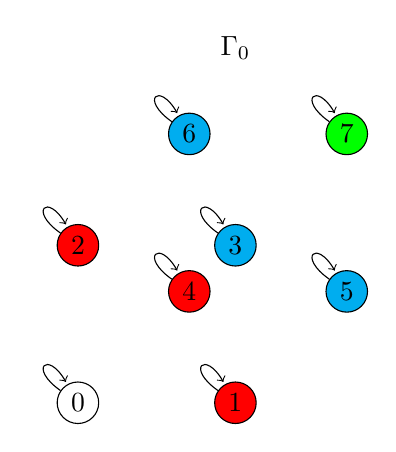
\begin{tikzpicture}[shorten >=1pt,auto,node distance=2cm,
		thin,main node/.style = {circle,draw, inner sep = 0pt, minimum size = 15pt}]
		
		\node[main node,fill=white] (1) {0};
		\node[main node,fill=red] [right of = 1](2) {1};
		\node[main node,fill=red] [above of = 1](3) {2};
		\node[main node,fill=cyan] [right of = 3](4) {3};
		\node[main node,fill=red] [above right of = 1](5) {4};
		\node[main node,fill=cyan] [right of = 5](6) {5};
		\node[main node,fill=cyan] [above of = 5] (7) {6};
		\node[main node,fill=green] [right of = 7](8) {7};
		\node at (2,4.5) (9) {$\Gamma_0$};
		
		\path (1) edge [in=120,out=145,loop] ();
		\path (2) edge [in=120,out=145,loop] ();
		\path (3) edge [in=120,out=145,loop] ();
		\path (4) edge [in=120,out=145,loop] ();
		\path (5) edge [in=120,out=145,loop] ();
		\path (6) edge [in=120,out=145,loop] ();
		\path (7) edge [in=120,out=145,loop] ();
		\path (8) edge [in=120,out=145,loop] ();
		
		\end{tikzpicture}\qquad&\qquad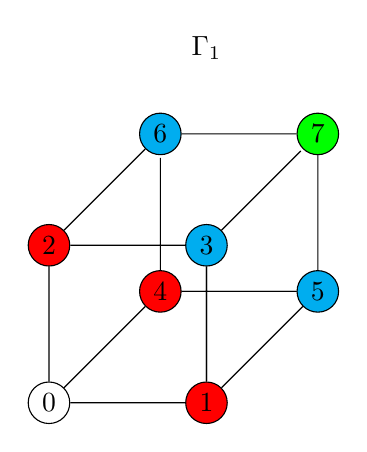
\begin{tikzpicture}[shorten >=1pt,auto,node distance=2cm,
		thin,main node/.style = {circle,draw, inner sep = 0pt, minimum size = 15pt}]
		
		\node[main node,fill=white] (1) {0};
		\node[main node,fill=red] [right of = 1](2) {1};
		\node[main node,fill=red] [above of = 1](3) {2};
		\node[main node,fill=cyan] [right of = 3](4) {3};
		\node[main node,fill=red] [above right of = 1](5) {4};
		\node[main node,fill=cyan] [right of = 5](6) {5};
		\node[main node,fill=cyan] [above of = 5] (7) {6};
		\node[main node,fill=green] [right of = 7](8) {7};
		\node at (2,4.5) (9) {$\Gamma_1$};
		
		\draw[-] (3)--(1)--(2)--(4)--(3)--(7)--(8)--(6)--(5)--(7);
		\draw[-] (1)--(5)--(6)--(2)--(4)--(8);
		\end{tikzpicture}\qquad\qquad
		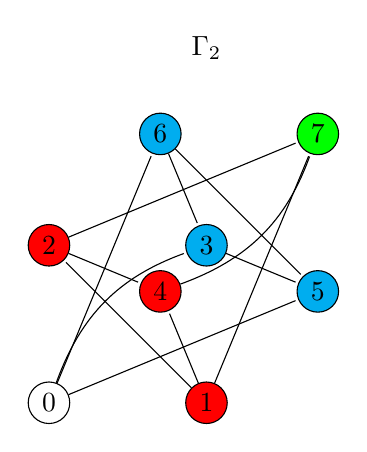
\begin{tikzpicture}[shorten >=1pt,auto,node distance=2cm,
		thin,main node/.style = {circle,draw, inner sep = 0pt, minimum size = 15pt}]
		
		\node[main node,fill=white] (1) {0};
		\node[main node,fill=red] [right of = 1](2) {1};
		\node[main node,fill=red] [above of = 1](3) {2};
		\node[main node,fill=cyan] [right of = 3](4) {3};
		\node[main node,fill=red] [above right of = 1](5) {4};
		\node[main node,fill=cyan] [right of = 5](6) {5};
		\node[main node,fill=cyan] [above of = 5] (7) {6};
		\node[main node,fill=green] [right of = 7](8) {7};
		\node at (2,4.5) (9) {$\Gamma_2$};
		
		\path[-]
		(1)edge [bend left=25] node {} (4)
		edge node {} (6)
		edge node {} (7)
		(2)edge node {} (3)
		edge node {} (5)
		edge node {} (8)
		(3)edge node {} (5)
		edge node {} (8)
		(4) edge node {} (6)
		(7) edge node {} (4)
		edge node {} (6)
		(5) edge [bend right = 25] node {} (8);
		\end{tikzpicture}\qquad&\qquad
		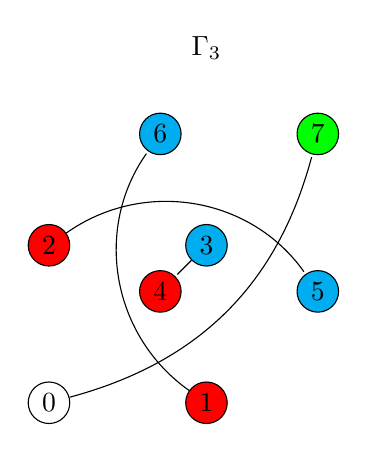
\begin{tikzpicture}[shorten >=1pt,auto,node distance=2cm,
		thin,main node/.style = {circle,draw, inner sep = 0pt, minimum size = 15pt}]
		
		\node[main node,fill=white] (1) {0};
		\node[main node,fill=red] [right of = 1](2) {1};
		\node[main node,fill=red] [above of = 1](3) {2};
		\node[main node,fill=cyan] [right of = 3](4) {3};
		\node[main node,fill=red] [above right of = 1](5) {4};
		\node[main node,fill=cyan] [right of = 5](6) {5};
		\node[main node,fill=cyan] [above of = 5] (7) {6};
		\node[main node,fill=green] [right of = 7](8) {7};
		\node at (2,4.5) (9) {$\Gamma_3$};
		
		\path[-]
		(1) edge [bend right] node {} (8)
		(2) edge [bend left=45] node {} (7)
		(3) edge [bend left=45] node {} (6)
		(4) edge node {} (5);
		\end{tikzpicture}
		\end{aligned}$}\end{center}
		\caption[Graphs of the 3-cube.]{The four graphs of the 3-cube. The four subconstituents of the vertex $0$ are colored white, red, blue, and green respectively.}\label{3cube}
		\end{figure}
		The following matrices give the intersection numbers of this association scheme where the $i^\text{th}$ matrix contains $p^k_{ij}$ with rows indexed by $k$ and columns indexed by $j$:
		\[\left[\begin{array}{cccc}
		1&0&0&0\\
		0&1&0&0\\
		0&0&1&0\\
		0&0&0&1\\
		\end{array}\right],\quad\left[\begin{array}{cccc}
		0&3&0&0\\
		1&0&2&0\\
		0&2&0&1\\
		0&0&3&0\\
		\end{array}\right],\quad\left[\begin{array}{cccc}
		0&0&3&0\\
		0&2&0&1\\
		1&0&2&0\\
		0&3&0&0\\
		\end{array}\right],\quad\left[\begin{array}{cccc}
		0&0&0&1\\
		0&0&1&0\\
		0&1&0&0\\
		1&0&0&0\\
		\end{array}\right].\]
		Since $p^k_{ij} = p^k_{ji}$, many of the columns listed above are redundant, thus we may instead give a more brief list of the intersection numbers as follows:
		\[\begin{array}{c|cccc|ccc|cc|c}
		k & p^{k}_{0,0}	&p^{k}_{0,1}& p^{k}_{0,2} 	& p^{k}_{0,3}   & p^{k}_{1,1}	&p^{k}_{1,2}& p^{k}_{1,3} 	& p^{k}_{2,2} 	& p^{k}_{2,3} 	& p^{k}_{3,3}\\\hline
		0 & 1			& 0			& 0 			& 0				& 3				& 0			& 0 			& 3				& 0   			& 1\\
		1 & 0			& 1			& 0 			& 0				& 0				& 2			& 0 			& 0   			& 1   			& 0\\
		2 & 0			& 0			& 1 			& 0				& 2				& 0 		& 1				& 2 			& 0 			& 0\\
		3 & 0			& 0			& 0 			& 1				& 0 			& 3			& 0 			& 0   			& 0 			& 0\\
		\end{array}\]
		We often find this brief description useful and will further reduce our description of the parameters when there is no loss of clarity.
		
		We note with this example that for each $i$, $\Gamma_i$ may be formed by taking the distance $i$ graph of $\Gamma_1$. This will not hold in general --- that is, we will typically not find such a graph encoding our relations using distance. When it does however, we say the association scheme is metric (see Section \ref{poly}) and $\Gamma_1$ is a distance-regular graph (drg). Due to the encoding of the relations in such a drg, metric schemes and their paired drgs are referred to synonymously; for instance, this association scheme was refereed to as the ``3-cube".
	\end{example}
	For any $0\leq i\leq d$ and any vertex $x\in X$,
	\[p^{0}_{ii} = \left\vert\left\{y:(y,x)\in R_i\right\}\right\vert = \left\vert R_i(x)\right\vert.\]
	Thus we define $k_i:=p^0_{ii}$ as the \emph{valency}\index{valency} of the $i^\text{th}$ relation. Many other restrictions on our intersection numbers follow immediately from our definition, for instance $p^0_{12} = 0$; we will summarize these in a lemma at the end of the next section.
	\section{Bose-Mesner algebra}\label{BMA}
	Often it becomes useful to order the vertices in $X$ and represent each $R_i$ as a 01-matrix $A_i$ where the $(x,y)$ entry of $A_i$ is 1 if and only if $(x,y)\in R_i$; thus $A_i$ is the adjacency matrix of $\Gamma_i$. Let $\vert X\vert = n$ and denote the $n\times n$ identity as $I_n$ and the $n\times n$ matrix of ones as $J_n$; we suppress the subscript $n$ when it is clear from the context. The defining properties of a symmetric association scheme are then encoded as:
	\begin{enumerate}[label=$(\roman*)$]
		\item $A_0 = I$;
		\item $\sum_i A_i = J$;
		\item for all $0\leq i\leq d$, $A_i^T = A_i$;
		\item for all $0\leq i,j\leq d$, $A_iA_j = \sum p_{ij}^k A_k$,
	\end{enumerate}
	where each $A_i$ has only zeros and ones as entries. The fourth condition tells us that $\BMA = \text{span}\left\{A_0,A_1,\dots A_d\right\}$ forms a matrix algebra under standard matrix multiplication --- we will refer to the matrices $\left\{A_i\right\}$ as our basis of 01-matrices\index{01-basis}. We call this algebra the \emph{Bose-Mesner algebra}\index{Bose-Mesner algebra} and note that the remaining conditions ensure it is a $(d+1)$-dimensional algebra of symmetric matrices containing the identity. Further, as our basis matrices are 01-matrices with pairwise disjoint support, this algebra is also closed under Schur (entrywise) products and contains the Schur identity, $J$. We find that, conversely, any such an algebra determines an association scheme; that is, any $(d+1)$-dimensional vector space of symmetric matrices closed under both standard and Schur matrix products containing the identities for both operations corresponds to the Bose-Mesner algebra of some symmetric association scheme. Throughout, we will use this algebraic definition interchangeably with the combinatorial definition. As our algebra contains only symmetric matrices, it is necessarily commutative (more generally the assumption $p^k_{ij} = p^k_{ji}$ made for commutative association schemes is sufficient to guarantee the Bose-Mesner algebra is commutative). Therefore, we may simultaneously diagonalize the matrices $A_0,\dots,A_d$ resulting in the maximal common orthogonal eigenspaces $V_0,\dots,V_{d'}$ with corresponding projection matrices $E_0,\dots,E_{d'}$. Since, for every $i$, there exist eigenvalues $\theta_{ij}$ such that $A_i = \sum_{j=0}^{d'}\theta_{ij}E_j$ we find that $\BMA \subseteq \text{span}\left\{E_0,E_1,\dots, E_{d'}\right\}$ thus $d\leq d'$. Further since the eigenspaces $V_j$ are maximal for each $0\leq j\leq d$ and pairwise orthogonal,
	\[E_j = \frac{1}{c_j}\prod_{i=0}^d\left(\prod_{\theta_{ik}\neq\theta_{ij}}\left(A_i-\theta_{ik}I\right)\right)\]
	for some normalization constant $c_j$. Thus each $E_j\in \BMA$ giving $\text{span}\left\{E_0,E_1,\dots, E_{d'}\right\}\subseteq\BMA$ and therefore $d=d'$ --- we will refer to the matrices $\left\{E_j\right\}$ as our basis of idempotents\index{idempotent basis}. This shows that $\BMA$ contains a basis of $d+1$ idempotents $E_0,\dots,E_d$ which together diagonalize every matrix in $\BMA$ and act as projection matrices onto the common eigenspaces. Since the rank 1 matrix $J\in\BMA$, we find that $\frac{1}{\vert X\vert}J$ must belong to this basis; by convention we assume $E_0= \frac{1}{\vert X\vert}J$. For each $0\leq j\leq d$ we define $m_j = \text{rank } E_j$ and note that $m_0 = 1$ and $\sum_{j=0}^dm_j = \vert X\vert$.
	
	While $\BMA = \text{span}\left\{A_0,A_1,\dots A_d\right\} = \text{span}\left\{E_0,E_1,\dots, E_{d}\right\}$, we often find that we may generate $\BMA$ with a single matrix if we allow ourselves to take products and not just linear combinations. For example, the Bose-Mesner algebra of the 3-cube (Example \ref{3cube}) may be generated by taking linear combinations of powers of $A_1$, the adjacency matrix of $\Gamma_1$. For any matrix $M\in\BMA$, we define $\left<M\right>_*$ as the set of matrices which are linear combinations of the powers of $M$; the set $\left<M\right>_*$ is called the \emph{subalgebra}\index{subalgebra} of $\BMA$ generated by $M$. 
	\begin{lem} \label{mstardim}
		Let $\BMA$ be the Bose-Mesner algebra of a symmetric association scheme. For any $A\in \BMA$, the dimension of $\left<A\right>_*$ equals the number of distinct eigenvalues.
	\end{lem}
	\begin{proof}
	Let $A\in \BMA$ be given with $n$ distinct eigenvalues. Then there exists $\alpha_1,\dots,\alpha_n$ so that $A = \sum_{i=1}^n\alpha_i E_i$ for some orthogonal projection matrices $E_1,\dots,E_n$ --- implying the dimension of $\left<A\right>_*$ is no larger than $n$. However, since $I = A^0$, we may build each $E_j$ via
	\[E_j = \frac{1}{c_j}\prod_{i\neq j} (A - \alpha_i I)\]
	showing that the dimension of $\left<A\right>_*$ is at least $n$.
	\end{proof}
	\begin{cor}
		For a Bose-Mesner algebra $\BMA$ and matrix $A\in \BMA$, $\BMA = \left<A\right>_*$ if and only if $A$ has $d+1$ distinct eigenvalues.
	\end{cor}
	Similarly, we define the \emph{Schur subalgebra}\index{subalgebra!Schur} of $M$, denoted $\left<M\right>_\circ$, as the set of matrices which are linear combinations of all Schur powers of $M$. We immediately see analogous results.
	\begin{lem} \label{mcircdim}
		Let $\BMA$ be the Bose-Mesner algebra of a symmetric association scheme. For any $E\in \BMA$, the dimension of $\left<E\right>_\circ$ equals the number of distinct entries in $E$.
	\end{lem}
	\begin{cor}
		For a Bose-Mesner algebra $\BMA$ and matrix $E\in \BMA$, $\BMA = \left<E\right>_\circ$ if and only if $E$ has $d+1$ distinct entries.
	\end{cor}
	As a simple example, it is clear that the subalgebra generated by any idempotent basis matrix (with two distinct eigenvalues) contains only multiples of that idempotent and the identity matrix. Similarly, the Schur subalgebra generated by any $01$-matrix contains only multiples of that $01$-matrix and any constant matrix ($cJ$ for some constant $c$). These specific subalgebras are typically not useful, thus we will typically only consider subalgebras of $01$-matrices and Schur subalgebras of idempotent matrices. For a more interesting example, consider again the 3-cube in Example 2.1. Let $A_i$ be the adjacency matrix of $\Gamma_i$ and note that $\left<A_1\right>_* = \BMA$ while $\left<A_2\right>_* = \left<A_0,A_2\right>$; that is, $A_1$ generates the entire Bose-Mesner algebra while $A_2$ generates a proper subset of $\BMA$. While not listed in the example, we find that this association scheme contains a single minimal idempotent whose Schur subalgebra equals $\BMA$ --- all other minimal idempotents generate a proper subset of $\BMA$. Throughout this thesis we will consider cases where the (Schur) subalgebra of a single matrix is the entire Bose-Mesner algebra (for instance, polynomial schemes) as well as others where the (Schur) subalgebra of some matrix is a proper subset of the Bose-Mesner algebra (for instance, imprimitive schemes) --- both situations may give rise to useful structure.
	
	We take a moment here to remark on the notion of duality in our matrix algebra. We have already mentioned that $\BMA$ is closed under two distinct products: standard matrix multiplication and Schur multiplication. While it is clear these are distinct products, they are indistinguishable at the formal level. Consider an abstract inner product space which admits a set of orthogonal basis vectors $\left\{b_i\right\}$ under the product $\star$. For any pair of vectors $v = \sum_i v_ib_i$ and $w = \sum_i w_ib_i$, we may define the \emph{product with respect to basis $\left\{b_i\right\}$} as $v\star w = \sum_i (v_iw_i)b_i$. In this light, the two products used in association schemes become very similar. Returning to our Bose-Mesner algebra, let $F,F'\in\BMA$ with $F = \sum_if_iE_i = \sum_i g_iA_i$ and $F' = \sum_if_i'E_i = \sum_i g_i'A_i$. We then find
	\[\begin{aligned}
	FF' & =\sum_{i,j}f_if_j'E_iE_j = \sum_i f_if_i'E_i;\qquad
	F\circ F' &=\sum_{i,j}g_ig_i'A_i\circ A_j= \sum_i g_ig_i'A_i.
	\end{aligned}\]
	Thus our two products may be described as the product with respect to the basis $\left\{E_i\right\}$ (standard matrix multiplication) and the product with respect to the basis $\left\{A_i\right\}$ (entrywise multiplication). We consider these two products dual operations on our algebra and their basis matrices dual bases. Throughout this thesis, we will often investigate this duality and point out when there are differences and/or gaps in our understanding of the landscape.
	
	While the algebraic structure of either basis with respect to its corresponding product is trivial, the manner in which matrix products and entrywise products interact is more interesting. Our first tool for understanding this interaction is the change of basis matrix from one set of idempotents to the other. For any Bose-Mesner algebra, the \emph{first and second eigenmatrices}\index{eigenmatrices} are given by $P$ and $Q$ respectively so that
	\begin{equation}
	\label{PQmat}
	A_i = \sum_{j} P_{ji} E_j,\qquad E_j = \frac{1}{\vert X\vert} \sum_{i} Q_{ij}A_i.
	\end{equation}
	The name of these matrices arises from the fact that column $i$ of $P$ consists of the eigenvalues of $A_i$ while column $j$ of $Q$ gives the ``dual eigenvalues" of $\vert X\vert E_j$ --- eigenvalues with respect to the Schur product. Let $\Delta_m=\text{diag}(m_0,m_1,\dots,m_d)$ and $\Delta_k=\text{diag}(k_0,k_1,\dots,k_d)$ and the following two relations hold for our eigenmatrices:
	\begin{lem}[\cite{Brouwer1989}, First and second orthogonality relations] \label{orthorels}\index{eigenmatrices!orthogonality relations}The eigenmatrices of an association scheme satisfy
		\begin{equation}
		PQ = \vert X\vert I, \qquad \Delta_mP = Q^T\Delta_k.
		\end{equation}
	\end{lem}
	These relations generalize the orthogonality relations of a group.
	
	A second consideration for our dual bases is to compare the structure constants for each product with respect to each basis. While we used the existence of structure constants $p^k_{ij}$ to show that $\BMA$ is closed under matrix multiplication, closure under Schur products is seen from the fact that the $A_i$ are pairwise orthogonal idempotents. This implies the existence of structure constants for our second basis. Thus, for $0\leq i,j,k\leq d$ there exist constants $q^k_{ij}$ so that
	\begin{equation}E_i\circ E_j = \frac{1}{\vert X\vert}\sum_k q_{ij}^k E_k.\label{Emult}\end{equation}
	We call these constants the \emph{Krein parameters}\index{parameters!Krein} of the association scheme. We note here that, while there are many distinct parameters of any association scheme, there are many relations which reduce our parameter space. For instance, any strongly regular graph (2-class association scheme) contains two $3\times 3$ matrices $P$ and $Q$ along with 27 intersection numbers and 27 Krein parameters, resulting in 72 total parameters --- yet the parameters of a connected strongly regular graph may be uniquely determined by exactly three parameters. In fact, just within the intersection numbers of the form $p^0_{ij}$, only $d+1$ of the $(d+1)^2$ intersection numbers are non-zero. With this in mind, we list out the basic properties of the adjacency matrices and orthogonal idempotents as well as the relations on the parameters which help reduce our parameter space. While we will use the lemmas that follow throughout the thesis, we emphasize here the duality at play between the two bases as well as their structure constants. See Lemmas 2.1.1, 2.2.1, 2.3.1, and Theorem 2.3.2 in the book of Brouwer, Cohen, and Neumaier \cite{Brouwer1989} for proofs of Lemma \ref{kitchensink}.
	
	
	\newpage
	\begin{lem}\label{AElem} The adjacency matrices $A_0,\dots,A_d$ and minimal idempotents $E_0,\dots,E_d$ satisfy:
		\begin{multicols}{2}
			\begin{enumerate}
				\item[(i)] $\displaystyle{A_0 = I}$,
				\item[(ii)] $\displaystyle{A_i\circ A_j = \delta_{ij}A_i}$,
				\item[(iii)] $\displaystyle{\sum_i A_i = J}$,
				\item[(iv)] $\displaystyle{A_iA_j = \sum_k p^k_{ij} A_k}$,
				\item[(v)] $\displaystyle{A_iE_j = P_{ji}E_j}$,\vfill\null
				\item[$(i')$] $\displaystyle{E_0 = J}$,
				\item[$(ii')$] $\displaystyle{E_iE_j = \delta_{ij}E_j}$,
				\item[$(iii')$] $\displaystyle{\sum_j E_j = I}$,
				\item[$(iv')$] $\displaystyle{\vert X\vert E_i\circ E_j = \sum_k q^k_{ij}E_k}$,
				\item[$(v')$] $\displaystyle{\vert X\vert A_i\circ E_j = Q_{ij} A_i}$.\vfill\null
			\end{enumerate}
		\end{multicols}
	\end{lem}
	
	\begin{lem}[{\cite{Brouwer1989}}]\label{kitchensink} The parameters $p^\ell_{ij}$, $q^\ell_{ij}$, $k_i = p^0_{ii}$, $m_j = q^0_{jj}$, and the eigenmatrices $P$ and $Q$ satisfy:
		\begin{multicols}{2}
		\begin{enumerate}
			\item[(i)] $\displaystyle{p_{0j}^\ell = \delta_{j\ell}}$,
			\item[(ii)] $\displaystyle{p^0_{ij} = \delta_{ij}k_i}$,
			\item[(iii)] $\displaystyle{p^\ell_{ij} = p^\ell_{ji}}$,
			\item[(iv)] $\displaystyle{p^\ell_{ij}k_\ell= p^j_{i\ell}k_j}$,
			\item[(v)] $\displaystyle{\sum_jp^\ell_{ij} = k_i}$,
			\item[(vi)] $\displaystyle{\sum_\ell p^\ell_{ij}p^m_{\ell h} = \sum_\ell p^m_{i\ell}p^\ell_{jh}}$,
			\item[(vii)] $\displaystyle{P_{ij}P_{ih} = \sum_\ell p^\ell_{jh}P_{i\ell}}$,
			\item[(viii)] $\displaystyle{P_{ji}Q_{hj} = \sum_\ell p_{i\ell}^hQ_{\ell j}}$,
			\item[(ix)] $\displaystyle{\sum_{j}P_{ji} = \sum_{h}p^h_{hi}}$,
			\item[(x)] $\displaystyle{P_{j0} = 1}$,
			\item[(xi)] $\displaystyle{P_{0i} = k_i}$,
			\item[(xii)] $\displaystyle{\sum_j m_jP_{ji}P_{jh} = \vert X\vert k_i\delta_{ih}}$,
			\item[(xiii)] $\displaystyle{p^\ell_{ij} = \frac{1}{\vert X\vert k_\ell}\sum_{h=0}^d m_hP_{hi}P_{h j}P_{h\ell}}$,
				
			\item[($i^\prime$)] $\displaystyle{q^\ell_{0j} = \delta_{j\ell}}$,
			\item[($ii^\prime$)] $\displaystyle{q^0_{ij} = \delta_{ij}m_j}$,
			\item[($iii^\prime$)] $\displaystyle{q^{\ell}_{ij} = q^\ell_{ji}}$,
			\item[($iv^\prime$)] $\displaystyle{q^\ell_{ij}m_\ell = q^j_{i\ell}m_j}$,
			\item[($v^\prime$)] $\displaystyle{\sum_j q^\ell_{ij} = m_i}$,
			\item[($vi^\prime$)] $\displaystyle{\sum_\ell q^\ell_{ij}q^{m}_{\ell h} = \sum_\ell q^m_{i\ell}q^\ell_{jh}}$,
			\item[($vii^\prime$)] $\displaystyle{Q_{ij}Q_{ih} = \sum_{\ell}q^\ell_{jh}Q_{i\ell}}$,
			\item[($viii^\prime$)] $\displaystyle{P_{ij}Q_{jh} = \sum_\ell q^i_{h\ell}P_{\ell j}}$,
			\item[($ix^\prime$)] $\displaystyle{\sum_{j}Q_{ji} = \sum_{h}q^h_{hi}}$,
			\item[($x^\prime$)] $\displaystyle{Q_{i0} = 1}$,
			\item[($xi^\prime$)] $\displaystyle{Q_{0j} = m_j}$,
			\item[($xii^\prime$)] $\displaystyle{\sum_i k_iQ_{ij}Q_{ih} = \vert X\vert m_j\delta_{jh}}$,
			\item[($xiii^\prime$)] $\displaystyle{q^\ell_{ij} = \frac{1}{\vert X\vert m_\ell}\sum_{h=0}^d k_hQ_{hi}Q_{h j}Q_{h\ell}}$.
			
		\end{enumerate}
		\end{multicols}
	\end{lem}
	We note that using this lemma, we find that any of the sets $\left\{p^k_{ij}\right\}_{i,j,k}$, $\left\{q^k_{ij}\right\}_{i,j,k}$, $\left\{P_{ij}\right\}_{i,j}$, or $\left\{Q_{ij}\right\}_{i,j}$ may be used to determine all the others. We define the collection of all four of these sets to be the \emph{parameter set}\index{parameter set} of an association scheme, noting immediately that it suffices to give any one of the four.
	\section{Parameter arrays}
	For a matrix $A$, we denote the entry in row $i$ and column $j$ as $\left[A\right]_{ij}$. We define the \emph{arrays of intersection numbers}\index{parameters!arrays of intersection numbers} $L_0,\dots,L_d$ as $(d+1)\PLH(d+1)$ matrices with $\left[L_i\right]_{kj} = p^k_{ij}$. We then define the vector space $\bbL = \text{span}\left\{L_0,\dots,L_d\right\}$ and note that Lemma \ref{kitchensink} \emph{(vi)} gives us
	\[
	\left[L_iL_j\right]_{mk} = \sum_\ell p^m_{i\ell }p^\ell_{jk} = \sum_{\ell }p^\ell_{ij}p^m_{\ell k} = \sum_\ell p^\ell_{ij}\left[L_\ell\right]_{mk}
	\]
	for $0\leq m,k\leq d$. Therefore we find that this vector space forms a matrix algebra under matrix multiplication with
	\begin{equation}\label{Lprod}
	L_iL_j = \sum_\ell p^\ell_{ij}L_\ell.
	\end{equation}
	Likewise, we define the \emph{arrays of Krein parameters}\index{parameters!arrays of Krein parameters} as $L_0^*,\dots,L_d^*$ with $\left[L_i^*\right]_{kj} = q^k_{ij}$. These span a dual matrix algebra $\bbL^* = \text{span}\left\{L_0^*,\dots,L_d^*\right\}$ as Lemma \ref{kitchensink} \emph{($\mathit{vi'}$)} gives
	\begin{equation}\label{Lstarprod}
	L_i^*L_j^* = \sum_{\ell}q^\ell_{ij}L_\ell^*.
	\end{equation}
	We now define algebra isomorphisms $\phi:\BMA\rightarrow\bbL$ and $\phi^*:\BMA\rightarrow\bbL^*$ via linear extension of the mappings
	\begin{equation}\label{algiso}
		\phi(A_i) = L_i,\qquad \phi^*(E_i) = \frac{1}{\vert X\vert}L_i^*.
	\end{equation}
	The first isomorphism preserves standard matrix multiplication while the second respects the Schur product in the sense that $\phi^*(M\circ N) = \phi^*(M)\phi^*(N)$. This provides us with the following lemma.
	\begin{lem}\label{arrayeigenvec}
		Let $P$ and $Q$ be the eigenmatrices of an association scheme with arrays of intersection numbers $L_0,\dots,L_d$ and arrays of Krein parameters $L_0^* ,\dots, L_d^*$. For each $0\leq i,j\leq d$, column $j$ of $Q$ is an eigenvector of $L_i$ with eigenvalue $P_{ji}$. Likewise column $i$ of $P$ is an eigenvector of $L_j^*$ with eigenvalue $Q_{ij}$.
	\end{lem}
	\begin{proof}
	Let $A_0,\dots,A_d$ be the 01-basis matrices and $E_0,\dots,E_d$ be the basis idempotents of our association scheme. Using Lemma \ref{AElem}, we recall that $A_i = \sum_{k} P_{ki}E_k$ and $E_iE_k = \delta_{ik}E_i$, thus $A_iE_j = P_{ji}E_j$. Applying $\phi$ to both sides of the equality $E_j = \frac{1}{\vert X\vert}\sum_{j}Q_{ji} A_i$ results in $\phi(\vert X\vert E_j) = \sum_{i}Q_{ij} L_i$ giving
	\[L_i\left(\sum_iQ_{ij}L_i\right) = \phi(A_i)\phi(\vert X\vert E_j)= \phi(\vert X\vert A_iE_j) = P_{ji}\left(\sum_iQ_{ij}L_i\right)  .\]
	 Similarly, we have $E_j = \frac{1}{\vert X\vert}\sum_{k} Q_{kj}A_k$ and $A_k\circ A_i = \delta_{ik}A_i$, thus $E_j\circ A_i = \frac{Q_{ji}}{\vert X\vert}A_i$. Now applying $\phi^*$ to both sides of $A_i = \sum_{j}P_{ji} E_j$ results in $\phi^*(\vert X\vert A_i) = \sum_{j}P_{ji} L_i^*$ giving
	\[L_j^*\left(\frac{1}{\vert X\vert}\sum_jP_{ji}L_j^*\right)=\phi^*(\vert X\vert E_j)\phi^*(A_j) = \phi^*(\vert X\vert E_j\circ A_i) =Q_{ji}\left(\frac{1}{\vert X\vert}\sum_jP_{ji}L_j^*\right).\]
	In each case, we note that $\left[L_i\right]_{j0} = \left[L_j^*\right]_{i0} = \delta_{ij}$ and thus column ``zero" of each matrix product gives our result.
	\end{proof}
	\begin{cor}
		Let $L_i$ ($L_j^*$) be an array of intersection numbers (Krein parameters) of a $d$-class association scheme. If $L_i$ ($L_j^*$) has $d+1$ distinct eigenvalues then it uniquely determines all remaining parameters of the scheme.
	\end{cor}
	\begin{proof}
		We will prove this for an array of intersection numbers, noting that the proof for an array of Krein parameters follows analogously. Let $L_i$ be an array of intersection numbers with $d+1$ distinct eigenvalues. First, $k_i = p^0_{ii} = [L_i]_{0i}$. We then use Lemma \ref{kitchensink} (iv) to solve for the valencies $k_0,\dots,k_d$. Now, since $L_i$ has $d+1$ distinct eigenvalues, we find $d+1$ distinct eigenvectors $v_0,\dots,v_d$ --- normalize these so that $(v_i)_0 = 1$ and define the matrix $M$ so that the $i^\text{th}$ column of $M$ is $v_i$. From Lemma $\label{arrayeigenvec}$, we know that the columns of $Q$ are exactly $m_iv_i$ where $m_i$ is the multiplicity of the given eigenvalue, thus $Q = M\Delta_m$. Thus, we must determine these multiplicities to finish our proof. However, Lemma \ref{orthorels} tells us that
		\[\begin{aligned}
		\vert X\vert \Delta_m = Q^T\Delta_k Q  = \Delta_m M^T\Delta_k M\Delta_m\\
		\end{aligned}\]
		Noting that all matrices given are invertible since each $k_i$ and $m_i$ are strictly positive, this gives $m_i = \bigslant{\vert X\vert}{v_i^T\Delta_kv_i}$.
	\end{proof}
	When relation $R_1$ is distinguished or projection matrix $E_1$ is distinguished, we refer to $L_1$ as the \emph{intersection matrix}\index{parameters!intersection matrix} and $L_1^*$ as the \emph{Krein matrix}\index{parameters!Krein matrix}; these two matrices will become particularly important for polynomial schemes (see Section \ref{poly}), for which they are tridiagonal. We end this section by noting that the matrices given in Example \ref{3cube} are exactly the arrays of intersection numbers for that association scheme. A final note before moving on is that the parameters of an association scheme need not define the scheme uniquely. In fact, there exist non-isomorphic $2$-class association schemes with exactly the same parameter set; consider the $4\times 4$ rook graph and the Shrikhande graph.
	\section{Formal duality of association schemes}\label{dualpair}
	In this section, we give an explicit example of the duality previously alluded to. Consider first the strongly regular graph $K_{3,3}$. This association scheme is a 2-class bipartite scheme with nontrivial relations given by adjacency in $K_{3,3}$ and non-adjacency in $K_{3,3}$ respectively. Thus the three graphs for this scheme are
		\begin{figure}[H]\begin{center}\scalebox{.7}{$\begin{aligned}
				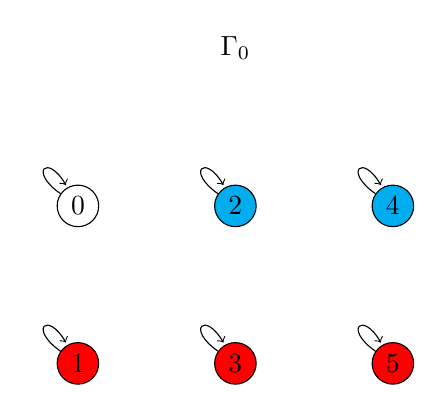
\begin{tikzpicture}[shorten >=1pt,auto,node distance=2cm,
				thin,main node/.style = {circle,draw, inner sep = 0pt, minimum size = 15pt}]
				
				\node[main node,fill=white] (1) {0};
				\node[main node,fill=cyan] [right of = 1](2) {2};
				\node[main node,fill=cyan] [right of = 2](3) {4};
				\node[main node,fill=red] [below of = 1](4) {1};
				\node[main node,fill=red] [right of = 4](5) {3};
				\node[main node,fill=red] [right of = 5](6) {5};
				\node [above of =2] (9) {$\Gamma_0$};
				
				\path (1) edge [in=120,out=145,loop] ();
				\path (2) edge [in=120,out=145,loop] ();
				\path (3) edge [in=120,out=145,loop] ();
				\path (4) edge [in=120,out=145,loop] ();
				\path (5) edge [in=120,out=145,loop] ();
				\path (6) edge [in=120,out=145,loop] ();
				
				\end{tikzpicture}\qquad&\qquad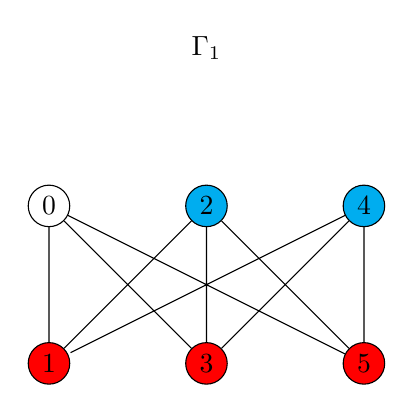
\begin{tikzpicture}[shorten >=1pt,auto,node distance=2cm,
				thin,main node/.style = {circle,draw, inner sep = 0pt, minimum size = 15pt}]
				
				\node[main node,fill=white] (1) {0};
				\node[main node,fill=cyan] [right of = 1](2) {2};
				\node[main node,fill=cyan] [right of = 2](3) {4};
				\node[main node,fill=red] [below of = 1](4) {1};
				\node[main node,fill=red] [right of = 4](5) {3};
				\node[main node,fill=red] [right of = 5](6) {5};
				\node [above of =2] {$\Gamma_1$};
				
				\draw[-] (1)--(4)--(2)--(5)--(3)--(6)--(1)--(5)--(2)--(6)--(3)--(4);
				\end{tikzpicture}\qquad\qquad
				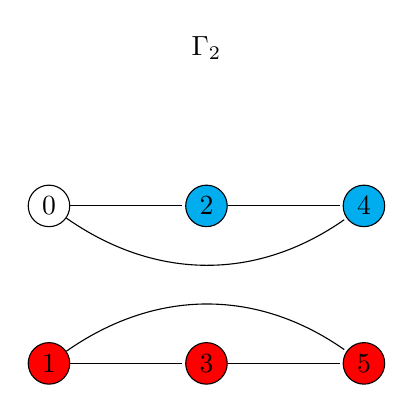
\begin{tikzpicture}[shorten >=1pt,auto,node distance=2cm,
				thin,main node/.style = {circle,draw, inner sep = 0pt, minimum size = 15pt}]	
				\node[main node,fill=white] (1) {0};
				\node[main node,fill=cyan] [right of = 1](2) {2};
				\node[main node,fill=cyan] [right of = 2](3) {4};
				\node[main node,fill=red] [below of = 1](4) {1};
				\node[main node,fill=red] [right of = 4](5) {3};
				\node[main node,fill=red] [right of = 5](6) {5};
				\node [above of =2] {$\Gamma_2$};
				
				\path[-]
				(1)edge node {} (2)
				edge [bend right=35] node {} (3)
				(2)edge node {} (3)
				(4)edge node {} (5)
				edge [bend left=35] node {} (6)
				(5) edge node {} (6);
				\end{tikzpicture}
				\end{aligned}$}\end{center}
		\caption[Graphs of $K_{3,3}$.]{The association scheme of $K_{3,3}$. The subconstituents of vertex $0$ are colored white, red,  and blue respectively.}\label{k33}
	\end{figure}
	The intersection numbers, Krein parameters, and eigenmatrices are
	\[\begin{aligned}L_0 &= \left[\begin{array}{cccc}
	1&0&0\\
	0&1&0\\
	0&0&1\\
	\end{array}\right],\quad L_1 &= \left[\begin{array}{cccc}
	0&3&0\\
	1&0&2\\
	0&3&0\\
	\end{array}\right],\quad L_2 &= \left[\begin{array}{cccc}
	0&0&2\\
	0&2&0\\
	1&0&1\\
	\end{array}\right];\\
	L_0^* &= \left[\begin{array}{cccc}
	1&0&0\\
	0&1&0\\
	0&0&1\\
	\end{array}\right],\quad L_1^* &= \left[\begin{array}{cccc}
	0&4&0\\
	1&2&1\\
	0&4&0\\
	\end{array}\right],\quad L_2^* &= \left[\begin{array}{cccc}
	0&0&1\\
	0&1&0\\
	1&0&0\\
	\end{array}\right];\end{aligned}\]
	\[P = \left[\begin{array}{rrr}
	1&3&2\\
	1&0&-1\\
	1&-3&2\\
	\end{array}\right],\qquad Q = \left[\begin{array}{rrr}
	1&4&1\\
	1&0&-1\\
	1&-2&1\\
	\end{array}\right].\]
	Now consider the $2$-class association scheme determined by the octahedron. The three graphs for this scheme are
	\begin{figure}[H]\begin{center}\scalebox{.7}{$\begin{aligned}
				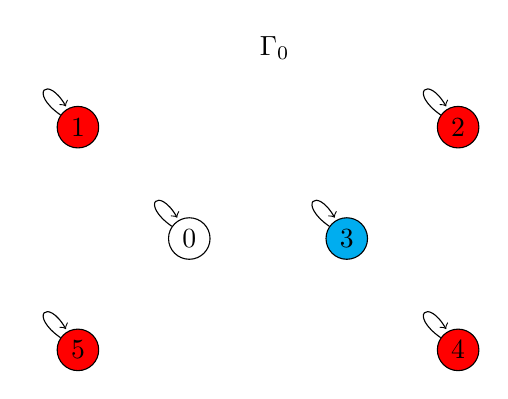
\begin{tikzpicture}[shorten >=1pt,auto,node distance=2cm,
				thin,main node/.style = {circle,draw, inner sep = 0pt, minimum size = 15pt}]
				
				\node[main node,fill=red] (2) {1};
				\node[main node,fill=white] [below right of = 2](1) {0};
				\node[main node,fill=cyan] [right of = 1](6) {3};
				\node[main node,fill=red] [above right of = 6](3) {2};
				\node[main node,fill=red] [below right of = 6](4) {4};
				\node[main node,fill=red] [below left of  = 1](5) {5};
				\node at (2.5,1) (9) {$\Gamma_0$};
				
				\path (1) edge [in=120,out=145,loop] ();
				\path (2) edge [in=120,out=145,loop] ();
				\path (3) edge [in=120,out=145,loop] ();
				\path (4) edge [in=120,out=145,loop] ();
				\path (5) edge [in=120,out=145,loop] ();
				\path (6) edge [in=120,out=145,loop] ();
				
				\end{tikzpicture}\qquad&\qquad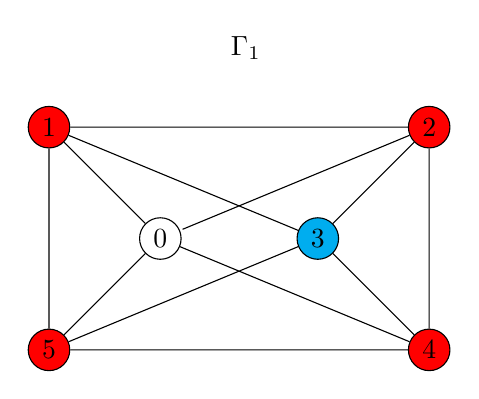
\begin{tikzpicture}[shorten >=1pt,auto,node distance=2cm,
				thin,main node/.style = {circle,draw, inner sep = 0pt, minimum size = 15pt}]
				
				\node[main node,fill=red] (2) {1};
				\node[main node,fill=white] [below right of = 2](1) {0};
				\node[main node,fill=cyan] [right of = 1](6) {3};
				\node[main node,fill=red] [above right of = 6](3) {2};
				\node[main node,fill=red] [below right of = 6](4) {4};
				\node[main node,fill=red] [below left of  = 1](5) {5};
				\node at (2.5,1) (9) {$\Gamma_1$};
				
				\draw[-] (1)--(2)--(3)--(4)--(5)--(2)--(6)--(5)--(1)--(4)--(6)--(3)--(1);
				\end{tikzpicture}\qquad\qquad
				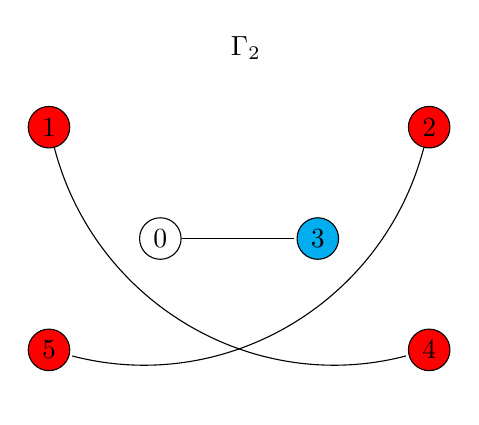
\begin{tikzpicture}[shorten >=1pt,auto,node distance=2cm,
				thin,main node/.style = {circle,draw, inner sep = 0pt, minimum size = 15pt}]	
				
				\node[main node,fill=red] (2) {1};
				\node[main node,fill=white] [below right of = 2](1) {0};
				\node[main node,fill=cyan] [right of = 1](6) {3};
				\node[main node,fill=red] [above right of = 6](3) {2};
				\node[main node,fill=red] [below right of = 6](4) {4};
				\node[main node,fill=red] [below left of  = 1](5) {5};
				\node at (2.5,1) (9) {$\Gamma_2$};
				
				\path[-]
				(1)edge node {} (6)
				(2)edge [bend right=45] node {} (4)
				(3)edge [bend left=45] node {} (5);
				\end{tikzpicture}
				\end{aligned}$}\end{center}
		\caption[Graphs of the octahedron.]{The association scheme of the octahedron. The subconstituents of vertex $0$ are colored white, red, and blue respectively.}\label{octahedron}
	\end{figure}
	The intersection numbers, Krein parameters, and eigenmatrices of this association scheme are
	\[\begin{aligned}
	L_0 &= \left[\begin{array}{cccc}
	1&0&0\\
	0&1&0\\
	0&0&1\\
	\end{array}\right],\quad L_1 &= \left[\begin{array}{cccc}
	0&4&0\\
	1&2&1\\
	0&4&0\\
	\end{array}\right],\quad L_2 &= \left[\begin{array}{cccc}
	0&0&1\\
	0&1&0\\
	1&0&0\\
	\end{array}\right];\\
	L_0^* &= \left[\begin{array}{cccc}
	1&0&0\\
	0&1&0\\
	0&0&1\\
	\end{array}\right],\quad L_1^* &= \left[\begin{array}{cccc}
	0&3&0\\
	1&0&2\\
	0&3&0\\
	\end{array}\right],\quad L_2^* &= \left[\begin{array}{cccc}
	0&0&2\\
	0&2&0\\
	1&0&1\\
	\end{array}\right];
	\end{aligned}\]
	\[P = \left[\begin{array}{rrr}
	1&4&1\\
	1&0&-1\\
	1&-2&1\\
	\end{array}\right],\qquad Q = \left[\begin{array}{rrr}
	1&3&2\\
	1&0&-1\\
	1&-3&2\\
	\end{array}\right].\]
	One may observe that the intersection numbers and the Krein parameters of the two schemes are interchanged, as are the first and second eigenmatrices. This specific example is due to a duality arising from the context of translation schemes and regular group actions. Given a point set $X$ and a group $G$, we say $G$ acts regularly on $X$ if, for any pair of points $x,y\in X$, there exists a unique $g$ mapping $x$ to $y$; clearly this may only occur if $\vert X\vert = \vert G\vert$. We then say an association scheme is a \emph{translation schemes}\index{translation schemes} if there is an abelian group acting regularly on the vertices such that for each $g\in \mathcal{G}$ and any pair of vertices $x,y\in X$, $(g(x),g(y))\in R_i$ if and only if $(x,y)\in R_i$. When this occurs, we may fix a vertex $x\in X$ and identify the remaining vertices with non-identity elements of $G$ corresponding to which element of $G$ maps $x$ to each vertex; thus we may identify $X$ with $G$ and consider our association scheme to be on the group $G$. The dual group $G^*$ is defined as the set of characters (homomorphisms mapping $G\rightarrow \mathbb{C}^*$) equipped with entrywise products as the group action. We then define the dual association scheme $(G^*,\mathcal{R}^*)$ where $(\chi,\chi')\in R_i^*$ if and only if $E_i\left(\bigslant{\chi}{\chi'}\right) = \left(\bigslant{\chi}{\chi'}\right)$ where this division is done entrywise. Finally, we find that the new association scheme is also a translation scheme using the group $\mathcal{G}^*$. In the case of the two association schemes given above, the desired group is $\mathcal{G}\simeq \bbZ_6$ and we find each scheme results as the dual of the other; in general we expect the dual operation to be an involution if the dual association scheme exists. The pair of schemes listed is a specific case of the more general duality between $\overline{rK_s}$ and $\overline{sK_r}$; that is, the complement of $r$ copies of $K_s$ and the complement of $s$ copies of $K_r$ respectively. In this more general setting, we find that the cyclic group $\bbZ_{rs}$ acts regularly on each set of vertices.
	
	In general, the automorphism group of an association scheme could be trivial. In this case, no group acts transitively on the vertices, and a dual scheme as described above is not defined. However, just as with non-linear codes in coding theory, we abstract the notion of duality to a formal definition on the parameters. We say two association schemes are \emph{formally dual}\index{formal duality} if the first and second eigenmatrices of one are the second and first eigenmatrices, respectively, of the other. This necessarily swaps the intersection numbers and Krein parameters so that, for example, $p^k_{ij}$ of a scheme will equal $q^k_{ij}$ of it's dual. In many cases, no formally dual scheme may exist; consider any association scheme for which the Krein parameters are not integral. However, there are non-trivial examples of formally dual pairs of association schemes, for instance consider the two infinite families generated by de Caen and van Dam \cite{deCaen1999}. This notion of formal duality still plays a major role in our understanding of the field of association schemes as a whole, motivating many of the questions we will focus on in this thesis.
	
	We finish this discussion with one final note: any definition based solely on the parameters of an association scheme gives rise to an analogous ``dual" definition. For instance, we find that $K_{3,3}$ is \emph{bipartite}\index{bipartite}, meaning $p^k_{ij}= 0$ whenever $i+j+k\notin2\bbZ$. The dual graph, the octahedron, must then have $q^k_{ij}=0$ whenever $i+j+k\notin2\bbZ$; we call this \emph{dual-bipartite}\index{bipartite!dual-} or $Q$-bipartite (see Section \ref{poly}). Similarly, we find that both $K_{3,3}$ and the octahedron are \emph{antipodal graphs}\index{antipodal}: $p^d_{di} = 0$ whenever $i\notin\left\{0,d\right\}$. Both graphs are then \emph{dual-antipodal}\index{antipodal!dual-} or $Q$-antipodal (see Section \ref{poly}): $q^d_{di}=0$ whenever $i\notin\left\{0,d\right\}$. While there has been much research into bipartite and antipodal graphs, in this thesis we are interested in the implications of these dual properties, seeking when such objects may exist and what combinatorial or geometric structure the properties impose.
	\section{Feasibility and realizability}
	One main point of interest is whether or not an association scheme exists, given a (possibly partial) parameter set. While existence often cannot be proven without explicitly constructing the scheme, we often may rule out the existence of a scheme due to the values its intersection numbers or Krein parameters must take. In this section we examine three main conditions which we will use throughout this thesis in addition to what we already stated in Lemma \ref{kitchensink}. We begin with an immediate restriction on the intersection numbers:
	\begin{lem}[\cite{Brouwer1989}]\label{intfeas}
		The intersection numbers of an association scheme must be non-negative integers.\qed
	\end{lem}
	This condition is easy to verify since, by definition, each $p^k_{ij}$ is the cardinality of a set. While this property is immediate, it can be a powerful tool to eliminate examples with very little information about the association scheme. Next consider the Krein parameters of our association scheme.
	\begin{lem}[\cite{Scott1973},Krein conditions]\label{kreinfeas}\index{Krein conditions}
		The Krein parameters of an association scheme must be non-negative real numbers.
	\end{lem}
	\begin{proof}
		Given a matrix $M$, let $\sigma(M)$ be the set of eigenvalues of $M$. From Equation \eqref{Emult}, we find that $\sigma(E_i\circ E_j) = \left\{\bigslant{q_{ij}^0}{\vert X\vert},\dots,\bigslant{q_{ij}^d}{\vert X\vert}\right\}$. However $E_i\circ E_j\in \BMA$ and therefore it must be symmetric, implying all of its eigenvalues are real. Further, note that $\sigma(E) = \left\{0,1\right\}$ for any projection matrix $E$. We also note that $\sigma(A\otimes B) = \left\{\alpha\beta,\alpha\in\sigma(A),\beta\in\sigma(B)\right\}$ for any pair of matrices $A$ and $B$. Thus, $\sigma(E_i\otimes E_j) = \left\{0,1\right\}$. Finally, since $E_i\circ E_j$ is a principal submatrix of $E_i\otimes E_j$, the eigenvalues of $E_i\circ E_j$ must be contained in the interval $0\leq \lambda\leq 1$.
	\end{proof}
	The final feasibility condition we will list here is known as the \emph{absolute bound}\index{absolute bound}.
	\begin{lem}[\cite{Neumaier1981},Absolute bound]\label{absolute}
		The multiplicities $m_i$ ($0\leq i\leq d$) of a $d$-class association scheme satisfy:
		\[\sum_{q_{ij}^k\neq 0} m_k\leq\begin{cases}
		m_im_j & \text{ if }i\neq j\\
		\binom{m_i+1}{2} & \text{ if }i= j.
		\end{cases}\]
	\end{lem}
	\begin{proof}
		The sum on the left is the rank of $E_i\circ E_j$, a principal submatrix of the rank $m_im_j$ matrix $E_i\otimes E_j$. Further, if $i=j$, $E_i\circ E_j$ is the entrywise square of $E_i$. Assuming $\text{col}(E_i) = \text{span}(v_1,\dots,v_{m_i})$, the columns of $E_i\circ E_i$ must be linear combinations of the vectors $v_j\circ v_k$ for $1\leq j\leq k\leq d$, a total of $\binom{m_i+1}{2}$ vectors.
	\end{proof}
	There are many other feasibility conditions we may list here including some arising from design theory and others as simple as the handshaking lemma. In this thesis however, we consider the conditions already stated to be a baseline. Thus, we do not claim that any parameter set fulfilling these conditions is guaranteed to correspond to the parameters of some association scheme, rather we instead simply ignore parameter sets which do not fulfill these basic parameter restrictions. We therefore define two separate terms which will be used throughout this thesis, \emph{feasible parameter sets}\index{feasible parameter set} and \emph{realizable parameter sets}\index{realizable parameter set}. \label{FCpage}
	\begin{definition}
		A \emph{feasible parameter set} is a set of Krein parameters, intersection numbers, and eigenmatrices such that:
		\begin{itemize}
			\item[FC1:] The Krein parameters satisfy Lemmas \ref{kreinfeas} and \ref{kitchensink} \emph{($\mathit{i'}$) -- ($\mathit{xiii'}$)},
			\item[FC2:] The intersection numbers satisfy Lemmas \ref{intfeas} and \ref{kitchensink} \emph{(i) -- (xiii)},
			\item[FC3:] The integers $m_j = q^0_{jj}$ satisfy Lemma \ref{absolute}.
		\end{itemize}
	\end{definition}
	\begin{definition}
		A feasible parameter set is \emph{realizable} if there exists an association scheme $(X,\cR)$ with the given parameter set.
	\end{definition}
	\section{Imprimitivity}\label{imprimitivity}
	In group theory, one is often interested in learning about the subgroups of any given group. That is, given a finite group $G$, are there subsets of the vertices $S\subset G$ for which the subset is closed under the group product. When such a subset occurs, we say $S$ is a subgroup of $G$, denoted $S\leq G$. In some cases, namely when our subgroup $N\leq G$ is normal, we may define another subgroup called the quotient group: $\nicefrac{G}{N}$. In this context, we often think of $G$ being built out of the normal subgroup $N$ and the quotient group $\nicefrac{G}{N}$, even though we cannot necessarily recover $G$ from these two ingredients. This line of investigation arises naturally in association schemes through the notion of subschemes. Within any Bose-Mesner algebra $\BMA$, we often find smaller subspaces $\BMB\subset\BMA$ which are closed under both entrywise products and standard matrix products. While these smaller algebras are typically not Bose-Mesner algebras (they need not include both identities $I$ and $J$), we may find a mapping from $\BMB$ to a vector space on smaller matrices which does result in a new Bose-Mesner algebra. Given an association scheme $(X,\mathcal{R})$, a subscheme $(X',\left\{R'_i\right\})$ is a subset of the points $X'\subset X$ paired with the non-empty relations $\left\{R'_i\right\}$ where $R'_i = R_i\cap(X'\times X')$ which itself forms an association scheme. The subalgebra mapping in this case corresponds to taking the principal submatrix of each matrix in $\BMA$ obtained by restricting to the rows and columns corresponding to the points $X'$. Just as in the group case, where every group $G$ contains two trivial subgroups $\left\{e_G\right\}$ and $G$ itself, every Bose-Mesner algebra $\BMA$ contains trivial subspaces closed under both products such as $\left<I\right>$ and $\BMA$; these will be ignored for all that follows.
	
	In this section we will examine the analogue of a non-simple group, called an imprimitive scheme which admits not only a non-trivial subscheme, but a quotient scheme as well. Analogous to a non-simple group, we often think of the imprimitive scheme as being built out of these two smaller schemes. However, knowing both the quotient scheme and the subscheme is not sufficient to entirely determine the original scheme. This is, in part, due to the many different types of products which may be used to piece smaller schemes together. For instance, Song \cite{Song2002} indicates the many distinct association schemes on 12 points using the standard direct and wreath products. Additionally, Cameron and Bailey \cite{Bailey2005} introduce a third product, called the ``crested product", which is distinct, in general, from the other two.
	
	An association scheme $(X,\mathcal{R})$ is \emph{imprimitive}\index{imprimitive} if there exists a non-trivial union of relations $\cup_{i\in \mathcal{I}} R_i$ which forms an equivalence relation on $X\times X$; here, the only trivial unions are $\mathcal{I} = \left\{0\right\}$ and $\mathcal{I} = \left\{0,\dots,d\right\}$. Given an imprimitive association scheme, we call the set of equivalence classes a \emph{system of imprimitivity}\index{imprimitivity!system of -} --- noting that a system of imprimitivity is determined uniquely by the index set $\mathcal{I}$. An equivalent definition for imprimitivity is as follows: an association scheme is \emph{imprimitive} if there exists a non-trivial relation whose graph is disconnected. To see the equivalence of these two definitions, assume that $R_i$ is disconnected for $i\neq 0$. Then $\cI = \left\{j:p^j_{ii}\right\}$ yields a system of imprimitivity.
	
	In some cases, we may have multiple systems of imprimitivity in our association scheme. Consider Example \ref{3cube} and note that $\cI_1 = \left\{0, 2\right\}$ and $\cI_2 = \left\{0, 3\right\}$ both yield systems of imprimitivity yet $\cI_1$ results in two equivalence classes while $\cI_2$ gives four. Thus we must be careful to distinguish between distinct systems of imprimitivity for any given association scheme. In each case, we find that the size of any equivalence class is equal to the sum of the valencies $k_i$ $(i\in\cI)$; hence all equivalence classes have the same size for a given system of imprimitivity. In the example of the 3-cube, the size of each equivalence class for $\cI_1$ is $v_0+v_2 = 4$; likewise the size of each equivalence class for $\cI_2$ is $v_0+v_3 = 2$. For all that follows we denote the size of any given equivalence class by $r$ and then the number of equivalence classes by $w$ noting that $\vert X\vert = wr$. We now define the subscheme and quotient scheme of an imprimitive scheme. Note that there is no distinction made between a general subscheme and one which corresponds to a single fiber of a system of imprimitivity. To avoid confusion, we will henceforth only refer to subschemes which arise from systems of imprimitivity throughout this text.
	
	\begin{definition}
		Let $(X,\mathcal{R})$ be an imprimitive association scheme with system of imprimitivity $X_1,\dots, X_w$ with index set $\mathcal{I}$.
		\begin{itemize}
			\item[(i)] The ($j^\text{th}$) \emph{subscheme} of $(X,\mathcal{R})$ is $\left(X_j,\left\{R'_i\right\}_{i\in\mathcal{I}}\right)$ where $R'_i = R_i\cap (X_j\times X_j)$.\index{imprimitivity!subscheme}
			\item[(ii)] The \emph{quotient scheme} of $(X,\mathcal{R})$ is the association scheme $\left(\left\{X_1,\dots,X_w\right\},\left\{\tilde{R}_i\right\}\right)$ where $(X_i,X_j)\in \tilde{R}_k$ if and only if there exists $x\in X_i$, $y\in X_j$ with $(x,y)\in R_k$.\index{imprimitivity!quotient scheme}
		\end{itemize}
	\end{definition}
	Note that the subscheme and quotient scheme depend explicitly on the system of imprimitivity chosen. Thus, in cases where multiple systems of imprimitivity exist, we must be careful to distinguish which we are using. Thus, if multiple systems of imprimitivity occur, say with index sets $\mathcal{I}_1$ and $\mathcal{I}_2$, we will say ``the quotient scheme (or subscheme) corresponding to $\mathcal{I}_1$". Before moving to examples, we will provide a derivation of each using their Bose-Mesner algebras. We do this to illuminate the duality at play, referring the reader to numerous other sources for a combinatorial derivation (\cite{Brouwer1989},\cite{Rao1984},\cite{Cameron1978},\cite{Martin2007}). 
	
	We begin with the subscheme. Let $(X,\cR)$ be given with the system of imprimitivity $X_1,\dots,X_w$ with index set $\cI = \left\{0,i_1,\dots,i_s\right\}$ and fiber size $r$. Then $\left\{A_i\right\}_{i\in\cI}$ forms a basis for a second matrix algebra $\mathbb{B}\subset\BMA$ which is also closed under both matrix and Schur multiplication. We may order the vertices by equivalence classes so that every matrix in $\mathbb{B}$ is block diagonal with $w$ blocks of size $r\times r$. Further, \[\left[\sum_{i\in\cI}A_i\right]_{x,y} = \begin{cases}
	1 \text{ if there exists a }0\leq k\leq w\text{ with }x,y\in X_k,\\
	0 \text{ otherwise.}
	\end{cases}\]
	Each of these matrices will therefore be block diagonal matrices as the $(x,y)$ entry of each matrix will be 0 for $x\in X_i$ and $y\in X_j$ $(i\neq j)$. However, this tells us that for $i,j\in \cI$,
	
	\[A_iA_j = \left[\begin{array}{cccc}
	\phi_1(A_i)\phi_1(A_j) & 0 & \dots & 0\\
	0 & \phi_2(A_i)\phi_2(A_j) & \dots & 0\\
	\vdots & \vdots & \ddots & \vdots \\
	0 & 0 & \dots & \phi_w(A_i)\phi_w(A_j)
	\end{array}\right]\]
	where $\phi_\ell$ maps any matrix $A$ to the $\ell^\text{th}$ $r\times r$ diagonal block. Thus we have $w$ vector spaces which are all isomorphic to $\BMB$, in particular, each vector space is closed under matrix multiplication and entrywise products. In addition however, each of these vector spaces contain both $I$ and $J$ since $\phi_\ell(A_0) = I$ and $\phi_\ell(\sum_{i\in\cI}A_i) = J$ for any choice of $1\leq \ell\leq w$. Thus each of these vector spaces is a subscheme of $\BMA$.
	
	\begin{lem}\label{sub}
		Let $\BMA$ be the Bose-Mesner algebra of an imprimitive scheme with system of imprimitivity with $w$ fibers of size $r$ and index set $\cI$. Then (under an appropriate ordering of the vertices) $\sum_{i\in\cI} A_i = I_w\otimes J_r$ and the Bose-Mesner algebra of the subscheme, $\BMA'$, is isomorphic to the vector space of matrices $\left<A_i\right>_{i\in\cI}$.
	\end{lem}
	
	Before moving to the quotient scheme, we investigate the subscheme further. As before, we note that $\BMB$ is commutative, and thus we may simultaneously diagonalize all matrices in $\BMB$ giving the basis of minimal idempotents $\left\{E^\prime_{0'},E'_{1'},\dots,E'_{s'}\right\}$ (here, we use $j'$ to denote an index of the subscheme noting that, in general, $E'_{j'}$ will not necessarily be related to $E_j$). Since every maximal common eigenspace of $\BMB$ must be the direct sum of maximal eigenspaces in $\BMA'$, the dimension of any maximal common eigenspace in $\BMB$ must be a multiple of $w$. Then, since we have shown the rank $w$ matrix $I_w\otimes J_r\in\BMB$, we know that $\frac{1}{r}I_w\otimes J_r$ must be one minimal idempotent as it is has the minimum possible non-zero rank of any idempotent matrix in $\BMB$; without loss of generality we assume this is $E^\prime_{0'}$. Now, since each maximal common eigenspace of $\BMA$ must be common eigenspaces of $\BMB$, we must have that for each $0\leq i\leq d$, there exists a unique $j'\in\left\{0',\dots,s'\right\}$ such that $E_j'E_i = E_i$ --- that is, the maximal common eigenspaces of $\BMB$ partition those of $\BMA$. We therefore define for each $j'\in\left\{0',\dots,s'\right\}$ the set $\left\{i:E'_{j'}E_i = E_i \right\}$ giving $E'_{j'} = \sum_{i\in\textbf{j}'}E_i$; for ease of notation, we identify an index $j'$ with both an index of the subscheme and the corresponding set of indices of idempotents from the original scheme contributing to $E_{j'}$. This is to emphasize that the idempotents of $\BMA'$ come from a partition of the idempotents of $\BMA$ --- we will see a similar notation for quotient schemes where relations of the quotient scheme arise from a partition of the relations of $\BMA$.	
	
	Since matrix multiplication is preserved by our mapping, we find that for $i,j,k\in\cI$, $p^{\prime k}_{ij} = p^k_{ij}$ and thus the intersection numbers match our original scheme for indices within $\cI$. While Schur products are also preserved by $\psi_\ell$, recall that the idempotents of $\BMB$ were not the same as the idempotents of $\BMA$, thus we do not expect our Krein parameters to be preserved. Instead we must determine the parameters $q^{\prime k'}_{i'j'}$ so that 
	\[E_{i'}^\prime\circ E_{j'}^\prime = \frac{1}{\vert X_\ell\vert} \sum_{k'=0'}^{s'}q^{\prime k'}_{i'j'}E_{k'}^\prime.\]
	First, note that such constants must exist since $\mathbb{B}$ is closed under entrywise multiplication. Now, recalling that $E_i^\prime = \sum_{a\in\hat{i}} E_a$, we may multiply each side of the above equation by $E_h$ for some $0\leq h\leq d$ and find
	\[\frac{1}{\vert X\vert}\sum_{a\in\hat{i},b\in\hat{j}} q^h_{ab}E_h = \left(E_{i'}^\prime\circ E_{j'}^\prime\right)E_h = \frac{1}{\vert X_\ell\vert}q^{\prime k'}_{i'j'} E_h \]
	where $h\in k'$. Thus we find
	\begin{equation}q^{\prime k'}_{i'j'} = \frac{1}{w}\sum_{a\in i',b\in j'}q^h_{ab}\end{equation}
	for any $h\in k'$.
	
	We note that, while there exist algebra isomorphisms between any pair of subschemes, the $w$ distinct subschemes need not be combinatorially isomorphic; that is, while $\psi_i\circ\psi_j^{-1}$ maps $\BMA_j'\rightarrow \BMA_i'$, there need not be a bijection between $X_j\rightarrow X_i$ for which $\left(\gamma(x),\gamma(y)\right)\in R_i^\prime$ if and only if $(x,y)\in R_i^\prime$ (see \cite{Jaeger1998} for further discussion on the distinction between ``isomorphic" and ``combinatorially isomorphic"). We summarize this construction as follows.
	 

	 	
	We now consider the dual notion, the \emph{quotient scheme}, by swapping the roles of our adjacency matrices and idempotents in the above derivation. As the quotient scheme and subscheme arise in the same context, it should not be surprising that they are highly related. Thus, we will hold on to some of the notation we have already established: using $j'\in\left\{0',\dots,s'\right\}$ to denote an index of the subscheme as well as the set $\left\{i:E^\prime_{j'} E_i = E_i\right\}$. Now, observe that Lemma \ref{kitchensink} \emph{($\mathit{i'}$)} applied to any subscheme tells us that $q^{\prime k'}_{0'0'} = 0$ for any $k'\neq 0'$. Thus, our original scheme must have $q^k_{ab} = 0$ whenever $a,b\in0'$ and $k\notin0'$. We denote $\cJ = 0'$ and find that the set of matrices $\left\{E_j\right\}_{j\in\cJ}$ is then closed under entrywise multiplication. Therefore we have a third vector space of matrices $\BMC = \text{span}_{j\in\cJ}\left(E_j\right)$ closed under both matrix and Schur multiplication. This vector space will be isomorphic to the Bose-Mesner algebra of our quotient scheme just as $\BMB$ was isomorphic to each $\BMA'$, however we require more work to show this.	
	
	Without loss of generality assume that $\vert \cJ\vert = t+1$. Since Schur products are trivially commutative, we may guarantee the existence of Schur idempotents (01-matrices) which span our matrix algebra. Let $\left\{\tilde{A}_{\tilde{0}},\dots,\tilde{A}_{\tilde{t}}\right\}$ correspond to the set of minimal Schur idempotents in $\BMC$; that is, the idempotents contained in $\BMC$ which are not sums of other Schur idempotents in $\BMC$. These new idempotents correspond to the maximal common Schur-eigenspaces of $\BMC$. However, since $\BMC\subset\BMA$, each schur idempotent must be a sum of 01-matrices from $\BMA$. As before, for each index $\tilde{i}\in\left\{\tilde{0},\dots,\tilde{t}\right\}$ we define the set $\tilde{i} = \left\{j:\tilde{A}_{\tilde{i}}\circ A_j = A_j\right\}$ giving $\tilde{A}_{\tilde{i}} = \sum_{j\in\tilde{i}}A_j$. This immediately implies that $\tilde{A}_{\tilde{i}}E_k = 0$ for any $k\notin \cJ$. Then each $\tilde{A}_{\tilde{i}}$ may be diagonalized using only the $\left\{E_j\right\}_{j\in\cJ}$ giving,
	\[\tilde{A}_{\tilde{i}}(I_w\otimes J_r) = \tilde{A}_{\tilde{i}}\left(r\sum_{j\in \cJ} E_j\right) = r\tilde{A}_{\tilde{i}}.\] 
	
	Thus, each $A^\prime_i$ is a block matrix, constant on each block. This block form tells us that any Schur idempotent of $\BMC$ must have a multiple of $wr^2$ ones since there must be at least $r^2$ ones in each of the $w$ rows of blocks. Then $I_w\otimes J_r$ must be one of our minimal idempotents since $I_w\otimes J_r\in \BMC$ and it has exactly $wr^2$ ones; without loss of generality, we assume $\tilde{A}_{\tilde{0}} = I_w\otimes J_r$. Further, the block form of our 01-matrices tells us there exists matrices $\tilde{M}_{\tilde{i}}$ for $\tilde{i}\in\left\{\tilde{0},\dots,\tilde{t}\right\}$ such that $\tilde{A}_{\tilde{i}} = J_r\otimes \tilde{M}_{\tilde{i}}$ and we may define an algebra homomorphism $\tilde{\psi}$ mapping $\tilde{A}_{\tilde{i}}\mapsto \tilde{M}_{\tilde{i}}$ which preserves entrywise multiplication. We further find that
	\begin{equation}\tilde{\psi}\left(AB\right) = r\tilde{\psi}(A)\tilde{\psi}(B).\label{tildepsiprod}\end{equation}
	Then $\tilde{\psi}(A^\prime_0) = I$, $\tilde{\psi}\left(\sum_{i\in\cJ}A'_i\right) =J_w$, and Equation \eqref{tildepsiprod} gives us,
	\[\tilde{p}^{\tilde{k}}_{\tilde{i}\tilde{j}} = \frac{1}{r}\sum_{i\in\tilde{i},j\in\tilde{j}}p^k_{ij}\]
	for any choice of $k\in\tilde{k}$; this smaller algebra satisfies all the conditions of a Bose-Mesner algebra. Finally, since $\tilde{\psi}$ preserves entrywise products, we find that $\tilde{q}^k_{ij} = q^k_{ij}$ for $i,j,k\in\cJ$.
	\begin{lem}\label{quotient}
	Let $\BMA$ be the Bose-Mesner algebra of an imprimitive scheme with system of imprimitivity with $w$ fibers of size $r$ and index set $\cI$. Then there exists an index set $\cJ$ such that $\sum_{j\in\cJ} E_j = \frac{1}{r}\left(I_w\otimes J_r\right)$ and the Bose-Mesner algebra of the quotient scheme, $\tilde{\BMA}$, is isomorphic to the vector space of matrices $\left<E_j\right>_{j\in\cJ}$.
	\end{lem}	

	From the above two derivations we find that both the subscheme and the quotient scheme may be obtained by finding a subset of idempotents under one product which are closed under the second product. When this occurs we find a smaller matrix algebra which is isomorphic to a Bose-Mesner algebra on fewer vertices. Thus the only algebraic difference between a subscheme and the quotient scheme is simply which set of idempotents we begin with (or rather, with respect to which product we take idempotents for). Throughout this thesis we will use $\tilde{i}$ to describe an index of the quotient scheme and $i^\prime$ an index of the subscheme. Further $\cI$ and $\cJ$ will continue to denote the subset of indices for which
	\[\sum_{i\in\cI} A_i = I_w\otimes J_r = r\sum_{j\in\cJ} E_j.\]
	In particular, we also allow ourselves to designate a system of imprimitivity via the index set $\cJ$, ensuring from context that the meaning of the index set is clear.	Finally, we have a lemma concerning the eigenmatrices of the subscheme and quotient scheme.
	\begin{lem}[\cite{Brouwer2003},\cite{Martin2007}]\label{repeatedcols}
	Let $P$ and $Q$ be the first and second eigenmatrix of an imprimitive association scheme with a system of imprimitivity given by index sets $\cI$ and $\cJ$. Let $P^\prime$ be the first eigenmatrix of the subscheme and $\tilde{Q}$ be the second eigenmatrix of the quotient scheme. Then for any $i\in \cI$ and $j\in \cJ$ we have
	\[P^\prime_{k'i} = P_{ki},\qquad \tilde{Q}_{\tilde{h}j} = Q_{hj}\]
	where $k\in k'$ and $h\in\tilde{h}$.
	\end{lem}
	\begin{proof}
		Recall that each subscheme of $\BMA$ is found by mapping each matrix in $\left<A_i\right>_{i\in\cI}$ to the principal submatrix corresponding to one of the equivalence classes. However, since $\phi:\BMA\rightarrow\BMA'$ via this mapping preserves matrix products, we see that 
		\[ P'_{k'i}\phi(E'_{k'}) = \phi(A_i)\phi(E'_{k'})= \phi(A_iE'_{k'})  =P_{ki}\phi(E'_{k'})\]
		 for any choice of $i\in\cI$ and $k\in k'$. Similarly, the mapping $\tilde{\psi}:\BMA\rightarrow\tilde{\BMA}$ preserves entrywise products. Thus choosing any $j\in\cJ$ and $h\in\tilde{h}$ results in
		 \[Q_{\tilde{h}j}\phi(\tilde{A}_{\tilde{h}}) = \tilde{\psi}(E_{j}\circ \tilde{A}_{\tilde{h}}) = \tilde{\psi}(E_{j})\circ\tilde{\psi}(\tilde{A}_{\tilde{h}}) = \tilde{Q}_{hj}\tilde{\psi}(\tilde{A}_{\tilde{h}})\]
	\end{proof}
	We finish this section by providing an illustration of each type of system of imprimitivity, returning to the example of the $3$-cube. Recall that this association scheme had two systems of imprimitivity with index sets $\cI_1 = \left\{0, 2\right\}$ and $\cI_2 = \left\{0, 3\right\}$. We begin with $\cI_1 = \left\{0,2\right\}$ and display the components of $\Gamma_2$ below.
		\begin{center}\scalebox{.7}{$\begin{aligned}
				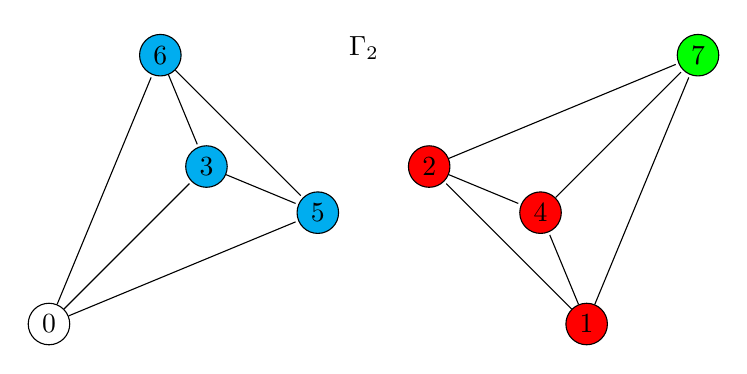
\begin{tikzpicture}[shorten >=1pt,auto,node distance=2cm,
				thin,main node/.style = {circle,draw, inner sep = 0pt, minimum size = 15pt}]
				
				\node[main node,fill=white] (1) {0};
				\node [right of = 1](2) {};
				\node [above of = 1](3) {};
				\node[main node,fill=cyan] [right of = 3](4) {3};
				\node [above right of = 1](5) {};
				\node[main node,fill=cyan] [right of = 5](6) {5};
				\node[main node,fill=cyan] [above of = 5] (7) {6};
				\node [right of = 7](8) {};
				
				\node [below right of =6] (11) {};
				\node[main node,fill=red] [right of = 11](12) {1};
				\node[main node,fill=red] [above of = 11](13) {2};
				\node [right of = 13](14) {};
				\node[main node,fill=red] [above right of = 11](15) {4};
				\node [right of = 15](16) {};
				\node [above of = 15] (17) {};
				\node[main node,fill=green] [right of = 17](18) {7};
				\node at (4,3.5) (9) {$\Gamma_2$};
				
				\path[-]
				(1)edge node {} (4)
				edge node {} (6)
				edge node {} (7)
				(12)edge node {} (13)
				edge node {} (15)
				edge node {} (18)
				(13)edge node {} (15)
				edge node {} (18)
				(4) edge node {} (6)
				(7) edge node {} (4)
				edge node {} (6)
				(15) edge node {} (18);
				\end{tikzpicture}
				\end{aligned}$}\end{center}
			For each of the two components we find a subscheme isomorphic to $K_4$:
		\begin{center}\scalebox{.7}{$\begin{aligned}
				\begin{tikzpicture}[shorten >=1pt,auto,node distance=2cm,
				thin,main node/.style = {circle,draw, inner sep = 0pt, minimum size = 15pt}]
				
				\node[main node,fill=white] (1) {0};
				\node[main node,fill=cyan] [right of = 3](4) {1};
				\node[main node,fill=cyan] [right of = 5](6) {2};
				\node[main node,fill=cyan] [above of = 5] (7) {3};
				\node at (2,4.5) (9) {$\Gamma_0^\prime$};
				
				\path (1) edge [in=120,out=145,loop] ();
				\path (4) edge [in=120,out=145,loop] ();
				\path (6) edge [in=120,out=145,loop] ();
				\path (7) edge [in=120,out=145,loop] ();
				
				\end{tikzpicture}\qquad\qquad
				\begin{tikzpicture}[shorten >=1pt,auto,node distance=2cm,
				thin,main node/.style = {circle,draw, inner sep = 0pt, minimum size = 15pt}]
				
				\node[main node,fill=white] (1) {0};
				\node[main node,fill=cyan] [right of = 3](4) {1};
				\node[main node,fill=cyan] [right of = 5](6) {2};
				\node[main node,fill=cyan] [above of = 5] (7) {3};
				\node at (2,4.5) (9) {$\Gamma_1^\prime$};
				
				\path[-]
				(1)edge node {} (4)
				edge node {} (6)
				edge node {} (7)
				(4) edge node {} (6)
				(7) edge node {} (4)
				edge node {} (6);
				\end{tikzpicture}
				\end{aligned}$}\end{center}
			The quotient scheme is found by collapsing each component to a single point, giving an association scheme isomorphic to $K_2$:
			\begin{center}\scalebox{.7}{$\begin{aligned}
			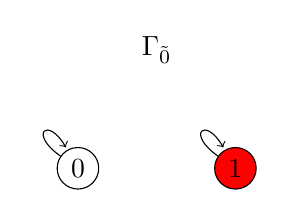
\begin{tikzpicture}[shorten >=1pt,auto,node distance=2cm,
			thin,main node/.style = {circle,draw, inner sep = 0pt, minimum size = 15pt}]
			
			\node[main node,fill=white] (1) {0};
			\node[main node,fill=red] [right of = 1](2) {1};
			\node at (1,1.5) (9) {$\Gamma_{\tilde{0}}$};
			
			\path (1) edge [in=120,out=145,loop] ();
			\path (2) edge [in=120,out=145,loop] ();
			
			\end{tikzpicture}\qquad\qquad
			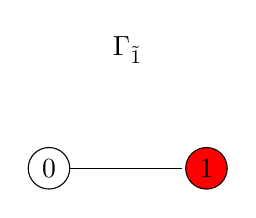
\begin{tikzpicture}[shorten >=1pt,auto,node distance=2cm,
			thin,main node/.style = {circle,draw, inner sep = 0pt, minimum size = 15pt}]
			
			\node[main node,fill=white] (1) {0};
			\node[main node,fill=red] [right of = 1](2) {1};
			\node at (1,1.5) (9) {$\Gamma_{\tilde{1}}$};
			
			\path[-]
			(1)edge node {} (2);
			\end{tikzpicture}
		\end{aligned}$}\end{center}
	Similarly, the system of imprimitivity corresponding to $\cI_2 = \left\{0,3\right\}$ results in the following components of $\Gamma_3$:
	\begin{center}\scalebox{.7}{$\begin{aligned}
			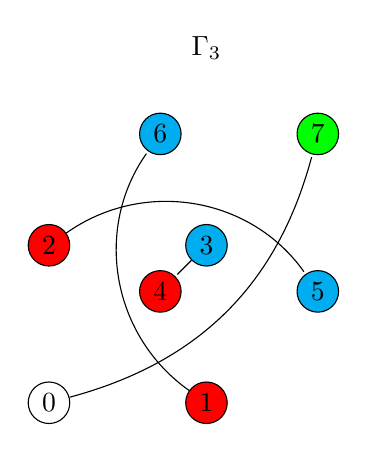
\begin{tikzpicture}[shorten >=1pt,auto,node distance=2cm,
			thin,main node/.style = {circle,draw, inner sep = 0pt, minimum size = 15pt}]
			
			\node[main node,fill=white] (1) {0};
			\node[main node,fill=red] [right of = 1](2) {1};
			\node[main node,fill=red] [above of = 1](3) {2};
			\node[main node,fill=cyan] [right of = 3](4) {3};
			\node[main node,fill=red] [above right of = 1](5) {4};
			\node[main node,fill=cyan] [right of = 5](6) {5};
			\node[main node,fill=cyan] [above of = 5] (7) {6};
			\node[main node,fill=green] [right of = 7](8) {7};
			\node at (2,4.5) (9) {$\Gamma_3$};
			
			\path[-]
			(1) edge [bend right] node {} (8)
			(2) edge [bend left=45] node {} (7)
			(3) edge [bend left=45] node {} (6)
			(4) edge node {} (5);
			\end{tikzpicture}
			\end{aligned}$}\end{center}
		Each component here results in a subscheme isomorphic to $K_2$:
		\begin{center}\scalebox{.7}{$\begin{aligned}
				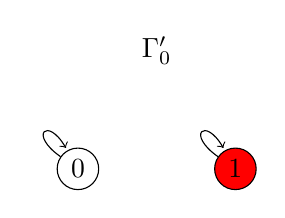
\begin{tikzpicture}[shorten >=1pt,auto,node distance=2cm,
				thin,main node/.style = {circle,draw, inner sep = 0pt, minimum size = 15pt}]
				
				\node[main node,fill=white] (1) {0};
				\node[main node,fill=red] [right of = 1](2) {1};
				\node at (1,1.5) (9) {$\Gamma_0^\prime$};
				
				\path (1) edge [in=120,out=145,loop] ();
				\path (2) edge [in=120,out=145,loop] ();
				
				\end{tikzpicture}\qquad\qquad
				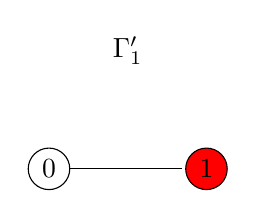
\begin{tikzpicture}[shorten >=1pt,auto,node distance=2cm,
				thin,main node/.style = {circle,draw, inner sep = 0pt, minimum size = 15pt}]
				
				\node[main node,fill=white] (1) {0};
				\node[main node,fill=red] [right of = 1](2) {1};
				\node at (1,1.5) (9) {$\Gamma_1^\prime$};
				
				\path[-]
				(1)edge node {} (2);
				\end{tikzpicture}
				\end{aligned}$}\end{center}
			while, the quotient scheme is isomorphic to $K_4$:
			
			\begin{center}\scalebox{.7}{$\begin{aligned}
					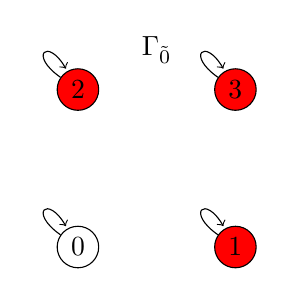
\begin{tikzpicture}[shorten >=1pt,auto,node distance=2cm,
					thin,main node/.style = {circle,draw, inner sep = 0pt, minimum size = 15pt}]
					
					\node[main node,fill=white] (1) {0};
					\node[main node,fill=red] [right of = 1](2) {1};
					\node[main node,fill=red] [above of = 1](3) {2};
					\node[main node,fill=red] [above of =2](4) {3};
					\node at (1,2.5) (9) {$\Gamma_{\tilde{0}}$};
					
					\path (1) edge [in=120,out=145,loop] ();
					\path (2) edge [in=120,out=145,loop] ();
					\path (3) edge [in=120,out=145,loop] ();
					\path (4) edge [in=120,out=145,loop] ();
					
					\end{tikzpicture}\qquad&\qquad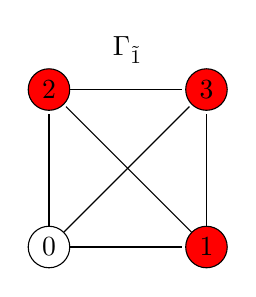
\begin{tikzpicture}[shorten >=1pt,auto,node distance=2cm,
					thin,main node/.style = {circle,draw, inner sep = 0pt, minimum size = 15pt}]
					
					\node[main node,fill=white] (1) {0};
					\node[main node,fill=red] [right of = 1](2) {1};
					\node[main node,fill=red] [above of = 1](3) {2};
					\node[main node,fill=red] [above of =2](4) {3};
					\node at (1,2.5) (9) {$\Gamma_{\tilde{1}}$};
					
					\path[-]
					(1) edge node {} (2)
					edge node {} (3)
					edge node {} (4)
					(2) edge node {} (3)
					edge node {} (4)
					(3) edge node {} (4);
					\end{tikzpicture}
					\end{aligned}$}\end{center}
	It is not typical that the two examples --- both in the same Bose-Mesner algebra --- have subscheme and quotient scheme swapped. This is an artifact of the self-duality of the 3-cube. These schemes correspond to the dual pair of linear codes $\text{rowsp}\left[\begin{array}{ccc}
	1 & 1 & 1
	\end{array}\right]$ and $\text{nullsp}\left[\begin{array}{ccc}
	1 & 1 & 1
	\end{array}\right].$
	\section{Polynomial schemes}\label{poly}
	In this section we define and briefly develop the notion of polynomial association schemes. We again present two dual concepts, $P$-polynomial and $Q$-polynomial, though we will focus primarily on the $Q$-polynomial case outside of this section. Let $(X,\cR)$ be a $d$-class association scheme. We say $(X,\cR)$ is \emph{$Q$-polynomial}\index{$Q$-polynomial}, or \emph{cometric}\index{$Q$-polynomial!cometric}, if there exists an ordering of the idempotents, say $E_0,E_1,\dots,E_d$, such that the Krein parameters satisfy the following conditions:
	\begin{enumerate}
		\item $q^k_{ij} = 0$ whenever $k>i+j$, and
		\item $q^k_{ij} > 0$ whenever $k = i+j$.
	\end{enumerate}
	Additionally, we note that it is sufficient to check only the above conditions with $i=1$ (see \cite[Prop.\ 2.7.1]{Brouwer1989}). Thus we may characterize $Q$-polynomial association schemes as exactly those for which there exists an eigenspace ordering for which the Krein matrix $L_1^*$ is irreducible tridiagonal. Noting that each row of $L_1^*$ sums to $q^0_{11}$, the parameters of $(X,\cR)$ are then entirely determined by its \emph{Krein array}\index{parameters!Krein array} $\iota^*(X,\cR) = \left\{b_0^*,\dots,b_{d-1}^*;c_1^*,\dots,c_d^*\right\}$ where $b_i^* = q^i_{1,i+1}$ and $c_i^* = q^{i+1}_{1i}$. When this occurs, we find that $\BMA = \left<E_1\right>_\circ$; that is, $E_1$ generates our entire Bose-Mesner algebra using Schur products. Additionally, for each $0\leq k\leq d$, we may define a single-variable polynomial $q_k(t)$ of degree $k$ so that $Q_{ik} = q_k\left(Q_{i1}\right)$ for $0\leq i\leq d$. This is equivalent to $E_k = \frac{1}{\vert X\vert}q_k\circ\left(\vert X\vert E_1\right)$; that is $q_k$ applied entrywise to $\vert X\vert E_1$ results in $\vert X\vert E_k$ (again see \cite[Prop.\ 2.7.1]{Brouwer1989}). Then we may define one final polynomial $q_{d+1}(t)$ with degree $d+1$ and no repeated roots such that $q_{d+1}\circ(\vert X\vert E_1) = 0$. This immediately implies that $E_1$ has $d+1$ distinct entries and we find it convenient to order the relations according to these values so that $Q_{01}>Q_{11}>\dots>Q_{d1}$; we call this the \emph{natural ordering of relations}\index{natural ordering} with respect to the $Q$-polynomial ordering $E_0,E_1,\dots,E_d$. As is suggested by this definition, it is possible to find multiple $Q$-polynomial orderings for the same association scheme. However, Suzuki \cite{Suzuki1998-2} showed that, with the exception of cycles, any $Q$-polynomial association scheme has at most two $Q$-polynomial orderings. We say a $Q$-polynomial association scheme is \emph{$Q$-bipartite}\index{$Q$-polynomial!$Q$-bipartite} if the Krein parameters satisfy $q^k_{ij} = 0$ whenever $i+j+k\notin 2\bbZ$. We find in this case that $\left\{E_i\right\}_{i\in 2\bbZ}$ serves as a Schur-closed subalgebra. In contrast, we say a $Q$-polynomial scheme is \emph{$Q$-antipodal}\index{$Q$-polynomial!$Q$-antipodal} if $q^k_{dd} = 0$ whenever $k\notin\left\{0,d\right\}$ and thus $\left\{E_0,E_d\right\}$ is a Schur-closed subalgebra. Each case coincides with a system of imprimitivity; the following is Suzuki's theorem concerning these systems.
	\begin{thm}[\cite{Suzuki1998},\cite{Cerzo2009},\cite{Tanaka2011}] \label{suzukiimprim} Suppose $(X,\mathcal{R})$ is an imprimitive cometric association scheme with $Q$-polynomial ordering $E_0,\dots,E_d$ and natural ordering $A_0,\dots,A_d$. Then one of the following holds:
	\begin{enumerate}[label=$(\roman*)$]
		\item $(X,\mathcal{R})$ is $Q$-bipartite and $\mathcal{J} = \left\{0,2,4,\dots\right\}$, $\mathcal{I} = \left\{0,d\right\}$;
		\item $(X,\mathcal{R})$ is $Q$-antipodal and $\mathcal{J} = \left\{0,d\right\}$, $\mathcal{I} = \left\{0,2,4,\dots\right\}$.
	\end{enumerate}
	\end{thm}
	The original theorem in \cite{Suzuki1998} allowed for two exceptional cases, one with $d=4$ and another with $d=6$. These two cases were later ruled out in \cite{Cerzo2009} and \cite{Tanaka2011} respectively.
	
	We now consider the more familiar dual notion: $P$-polynomial association schemes. Again let $(X,\cR)$ be a $d$-class association scheme. We say $(X,\cR)$ is \emph{$P$-polynomial}\index{$P$-polynomial}, or \emph{metric}\index{$P$-polynomial!metric}, if there exists an ordering of the relations, say $A_0,A_1,\dots,A_d$, such that the intersection numbers satisfy the following conditions:
	\begin{enumerate}
		\item $p^k_{ij} = 0$ whenever $k>i+j$, and
		\item $p^k_{ij} > 0$ whenever $k = i+j$.
	\end{enumerate}
	Just as with cometric association schemes, we find that it suffices to check the above conditions only when $i=1$ (\cite[Prop.\ 2.7.1]{Brouwer1989}) and thus an association scheme is $P$-polynomial if and only if there exists an ordering of the relations for which the intersection matrix $(L_1)$ is irreducible tridiagonal. In this case we find that $\BMA= \left<A_1\right>_*$ and it is therefore common to consider a $P$-polynomial scheme synonymous with $\Gamma_1$ --- a \emph{distance-regular graph}; that is $(x,y)\in R_i$ if and only if the distance between $x$ and $y$ in $\Gamma_1$ is $i$. We find analogous results as we saw in the $Q$-polynomial case with \cite[Theorem 4.2.12]{Brouwer1989} and \cite{Taylor1978} giving that any $P$-polynomial association scheme which is not a cycle has at most two $P$-polynomial orderings. Further, we may define \emph{$P$-bipartite}\index{$P$-polynomial!bipartite} (or more commonly \emph{bipartite}) and \emph{$P$-antipodal}\index{$P$-polynomial!antipodal} (\emph{antipodal}) as those schemes for which $p^k_{ij}= 0$ if $i+j+k\not\in 2\bbZ$ and $p^k_{dd}= 0$ whenever $k\not\in\left\{0,d\right\}$ respectively. For these schemes we again find systems of imprimitivity. This time, however, $\mathcal{I} = \left\{0,2,4,\dots\right\}$ and $\mathcal{J} = \left\{0,d\right\}$ corresponding to the bipartition of a bipartite graph, while $\mathcal{I} = \left\{0,d\right\}$ and $\mathcal{J} = \left\{0,2,4,\dots\right\}$ give the antipodal classes as our system. As before, with the exception of cycles, we find that these systems of imprimitivity are all that can occur for $P$-polynomial schemes and note that both can occur within the same association scheme, for example the $3$-cube (more generally the $n$-cube) is both bipartite and antipodal. For details, see Theorem 4.2.1 in the book \cite{Brouwer1989} of Brouwer, et al.\ where credit is given to Smith \cite{Smith1971} and Gardiner \cite{Gardiner1980} where this is reference ``313" in the book \cite{Brouwer1989}.
	
	Despite the close connection between $P$-polynomial and $Q$-polynomial association schemes, we note that many of the theorems mentioned here in the $P$-polynomial case predate their $Q$-polynomial analogues by as much as 30 years. Further, there are many other theorems which are known to be true for metric schemes whose cometric analogues have yet to be proven. For instance Taylor and Levingston showed in 1978 (\cite{Taylor1978}) that the sequence $k_0,k_1,\dots,k_d$ is unimodal, however the $Q$-analogue --- the property that the sequence $m_0,m_1,\dots,m_d$ is unimodal for any $Q$-polynomial ordering --- remains a conjecture to this day. Chapter 6 of \cite{Brouwer1989} details many of the known examples of distance-regular graphs --- all tables mentioned here appear in that chapter. Brouwer, et al.\ list 21 classical parameter sets (Tables 6.1 \& 6.2), 15 of which correspond to infinite families, three folded classical graphs (Table 6.3), nine near regular polygons including the generalized polygons (Tables 6.5 \& 6.6), as well as 20 more primitive distance regular graphs (Tables 6.8 \& 6.9). Further they give the known bipartite and antipodal examples (Tables 6.9 \& 6.10 resp.). On the cometric side however, much less is known. Out of the infinite families of $P$-polynomial schemes listed in \cite{Brouwer1989}, five families are also $Q$-polynomial: the Johnson schemes, Hamming schemes, Grassmann schemes, dual polar spaces, and sesquilinear/quadratic forms. More recently \cite{VanDam2005}, Van Dam and Koolen discovered the twisted Grassmann graphs which are also both metric and cometric. The remaining known families $Q$-polynomial association schemes are: linked systems of symmetric designs, mutually unbiased bases, bipartite doubles of some polar spaces, duals of metric translation schemes, two families found by Penttila and Williford \cite{Penttila2011} --- one 4-class $Q$-bipartite and one 3-class primitive --- and one more family found by Moorhouse and Williford \cite{Moorhouse2016}. In addition to these we also know of sporadic examples such as the 22 listed in \cite{Martin2007} and new examples found by King \cite{King2018}. Out of these examples, we note that only the families which are both metric and cometric allow for unbounded $d$. In fact, Bannai and Ito made the following conjecture concerning primitive association schemes.
	\begin{conj*}[Bannai \& Ito] 
		For $d$ sufficiently large, a primitive association scheme with $d$ classes is metric if and only if it is cometric.
	\end{conj*}
	We note that every primitive $2$-class association scheme (connected strongly regular graph) is vacuously both metric and cometric. Thus, in view of the above conjecture, it should not be surprising that the most fruitful place to search for new examples of $Q$-polynomial schemes which are not also metric is the range $3\leq d\leq 6$.